\documentclass[10pt,conference,onecolumn,compsoc]{IEEEtran}

\usepackage{hyperref}
\usepackage{enumitem}

\setlist[itemize]{leftmargin=3 cm}
\setlist[enumerate]{leftmargin=3cm}



% *** CITATION PACKAGES ***
%
\ifCLASSOPTIONcompsoc
  \usepackage[nocompress]{cite}
\else
  \usepackage{cite}
\fi



% *** GRAPHICS RELATED PACKAGES ***
%
\ifCLASSINFOpdf
   \usepackage[pdftex]{graphicx}
\else
\fi


% correct bad hyphenation here
\hyphenation{op-tical net-works semi-conduc-tor}


\begin{document}
%title
\title{Financial Planner}

%author names
\author{Cody Gonsowski\\ Trever Hall}% <-this % stops a space

% As a general rule, do not put math, special symbols or citations
% in the abstract or keywords.
\IEEEtitleabstractindextext{%
\begin{abstract}
This financial planner is meant to help users keep track of their spending habits. It can display expense and income information over an extended timeframe and allows the user to navigate to a specific day's information through a user interface. The target audience is anyone seeking to have more financial stability, but people can easily use it for casual financial tracking. We have made corrections as recommended by our instructor and added use cases, functional and non-functional requirements, and interface mockups. 
\end{abstract}
}


% make the title area
\maketitle


\IEEEdisplaynontitleabstractindextext
\IEEEpeerreviewmaketitle


\section{Introduction}

This is a financial planner that allows users to track expenses over time and create a budget. Most young adults, especially college students, have a hard time with money, either from a lack of funds or spending irresponsibly. If financial habits go unchecked, a person can get trapped in a vicious cycle of debt and high interest rates, just to afford to live. Even if people are not having a hard time with money, it still helps to develop good habits for the future as soon as possible.

The goal is to provide users with an outlet to track their expenses and plan a budget that allows them to live more comfortably within the income they have. By tracking and categorizing expenses, even all the small amounts, people will be able to see where their money goes and how much it adds up. Once people recognize how much they are actually spending, they are then able to tailor a budget to their needs.


\subsection{Background}
The primary goal of this project is to make users feel more secure with their financial decisions by allowing them to track expenses and income over time.  Expenses include any money spent on bills, groceries, personal items, etc. Income is all money accrued, regardless of its source (i.e., interest from investments or an earned wage). Users will be able to know where their funds are at any given time by being as specific and inclusive as possible.

We believe that not only will this project will be challenging but also it will provide something practical. Trever Hall, a developer on the team, uses a paperback financial planner to keep track of funds. He would like to have an online planner to use in his day-to-day life to manage his own finances.


\subsection{Challenges}
Because the program seems relatively straightforward, we are unsure of all the challenges to come. However, challenges we expect to come across include as follows: on-demand creation of custom expense and income categories, graphical interface that scales from years to a specific day, and gathering APIs we would like to use to help the user experience.

%As you overcome these challenges, this section becomes more of a retrospective: don't only identify the challenge, but also briefly outline the solution!


\section{Scope}
The user will be able to locate a specific day within a year. Once there, the user can view all information for that day and add expense and income information. The user will be able to add expenses and income to a selection of preset categories, as well as custom user-created categories. Expense and income information will be displayed alongside each other for easy comparison. Total money spent or earned in each category, as well as net income, will be displayed on every view implemented (yearly, monthly, etc.).

Some stretch goals we would like to implement to provide a better, more convenient user experience include as follows: graphical representation of data for the current view (i.e., categorical pie chart) and a fullscreen calendar that allows the user to navigate to a specific day (more aesthetic).

%add out of scope of this class goals?


\subsection{Requirements}
Each user should have their own planner independent from other users; by using an account-based system, this becomes very simple. When using accounts, however, security is something that cannot be overlooked. Ensuring that the planner scales well with large amounts of information allows for users to input data freely.

%explains how we got func and non-func requirements

\subsubsection{Functional}
\begin{itemize}
\item User needs to have a personal financial planner -- this will be on a per-user basis
\item Users will have accounts that allows them to access their own planner from anywhere with an internet connection and the appropriate software -- this allows users to remotely change their planner
\item Calendar date selection should be locked to only valid, calendar-standard, integer inputs
\end{itemize}

%add more functional requirements

\subsubsection{Non-Functional}
\begin{itemize}
\item Security -- user credentials must be encrypted on disk, users should be able to reset their passwords if forgotten
\item Scalability -- planner should be able to handle many years' worth of information
\end{itemize}


\subsection{Use Cases}
%This subsection is arguably part of how you define your project scope (why it is in the Scope section...).  In a traditional Waterfall approach, as part of your requirements gathering phase (what does the product actually \emph{need} to do?), you will typically sit down with a user to develop use cases.

%You should have a table listing all use cases discussed in the document, the ID is just the order it is listed in, the name should be indicative of what should happen, the primary actor is typically most important in an application where you may have different levels of users (think admin vs normal user), complexity is a best-guess on your part as to how hard it should be.  A lower number in priority indicates that it needs to happen sooner rather than later.  A sample table, or Use Case Index can be seen in Table \ref{tab:useCaseIndex}.

%use case table
\begin{table}
\centering
\begin{tabular}{|c|c|c|c|c|}
\hline
Use Case ID & Use Case Name & Primary Actor & Complexity & Priority \\
\hline \hline
1 & Search date & User & Med & 1\\
\hline
2 & Add budget category & User & Med & 1\\
\hline
3 & Sign-in & User & Med & 1\\
\hline

\end{tabular}
\caption{Use case table}
\label{tab:useCaseIndex}
\end{table}

%use cae 1
\begin{itemize}
\item[Use Case Number:] 1
\item[Use Case Name:] Search date
\item[Description:] A user enters the calendar date where they want to go. They will click on the "Search" button. This will adjust the calendar and info view accordingly.
\end{itemize}

\begin{enumerate}
\item User enters the month, day, and/or year they wish to jump to
\item User left-clicks on the "Search" button
\item Calendar and Info displays now display the chosen date and its information
\item[Termination Outcome:] The user's planner is updated to display information of the chosen date.
\end{enumerate}

%use case 1, alternative 1
Alternative: Input is invalid
\begin{enumerate}
\item User enters the month, day, and/or year they wish to jump to
\item User left-clicks on the "Search" button
\item Calendar and Info displays are reset to the previous selected date
\item[Termination Outcome:] The user's planner display is left unchanged.
\end{enumerate}

%use case 2
\begin{itemize}
\item[Use Case Number:] 2
\item[Use Case Name:] Add budget category
\item[Description:] A user would like to add a custom budget category. They will enter a custom category in the "Add a category" text box. They will click "Confirm." This will add a custom category for the budget section.
\end{itemize}

\begin{enumerate}
\item User enters the name of the category they would like to add into the "Add a category" text box
\item User left-clicks on the "Confirm" button
\item Budget should now have a new available category
\item[Termination Outcome:] The budget section should now have an additional category to add budget info under.
\end{enumerate}

%use case 3
\begin{itemize}
\item[Use Case Number:] 3
\item[Use Case Name:] Sign-in
\item[Precondition:] User already has a pre-existing account.
\item[Description:] A user wants to sign-in to access their financial planner. The user enters their username in the "Username" text box and their password in the "Password" text box. They will click "Sign-in." This will allow them to access their personal financial planner.
\end{itemize}

\begin{enumerate}
\item User enters their username into the "Username" text box
\item User enters their password into the "Password" text box
\item User left-clicks the "Sign-in" button
\item User can access their financial planner
\item[Termination Outcome:] The user should be signed in and able to access and edit their own unique financial planner.
\end{enumerate}

%use case 3, alternative 1
Alternative: User enters incorrect username or password
\begin{enumerate}
\item User enters their username into the "Username" text box
\item User enters their password into the "Password" text box
\item User left-clicks the "Sign-in" button
\item The username and password boxes reset to empty
\item[Termination Outcome:] The user is unable to sign in and needs to try again in order to access their unique financial planner.
\end {enumerate}

%\begin{figure}[ht!]
%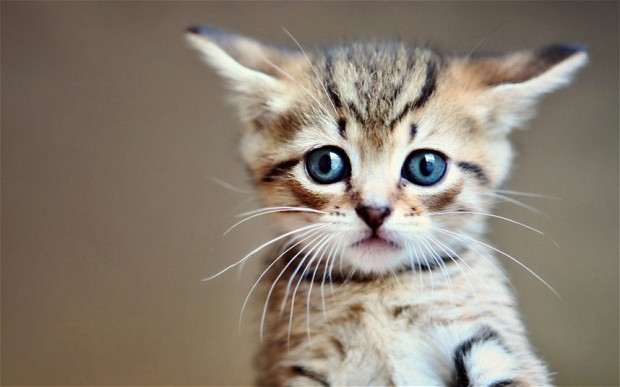
\includegraphics[height=250px, width=350px]{cat1.jpg}
%\caption{First picture, this is a kitten, not a use case diagram}
%\label{cat1}
%\end{figure}

\subsection{Interface Mockups}

\smallskip

\begin{figure}[h]
\centering
\begin{minipage}{.5\textwidth}
\centering
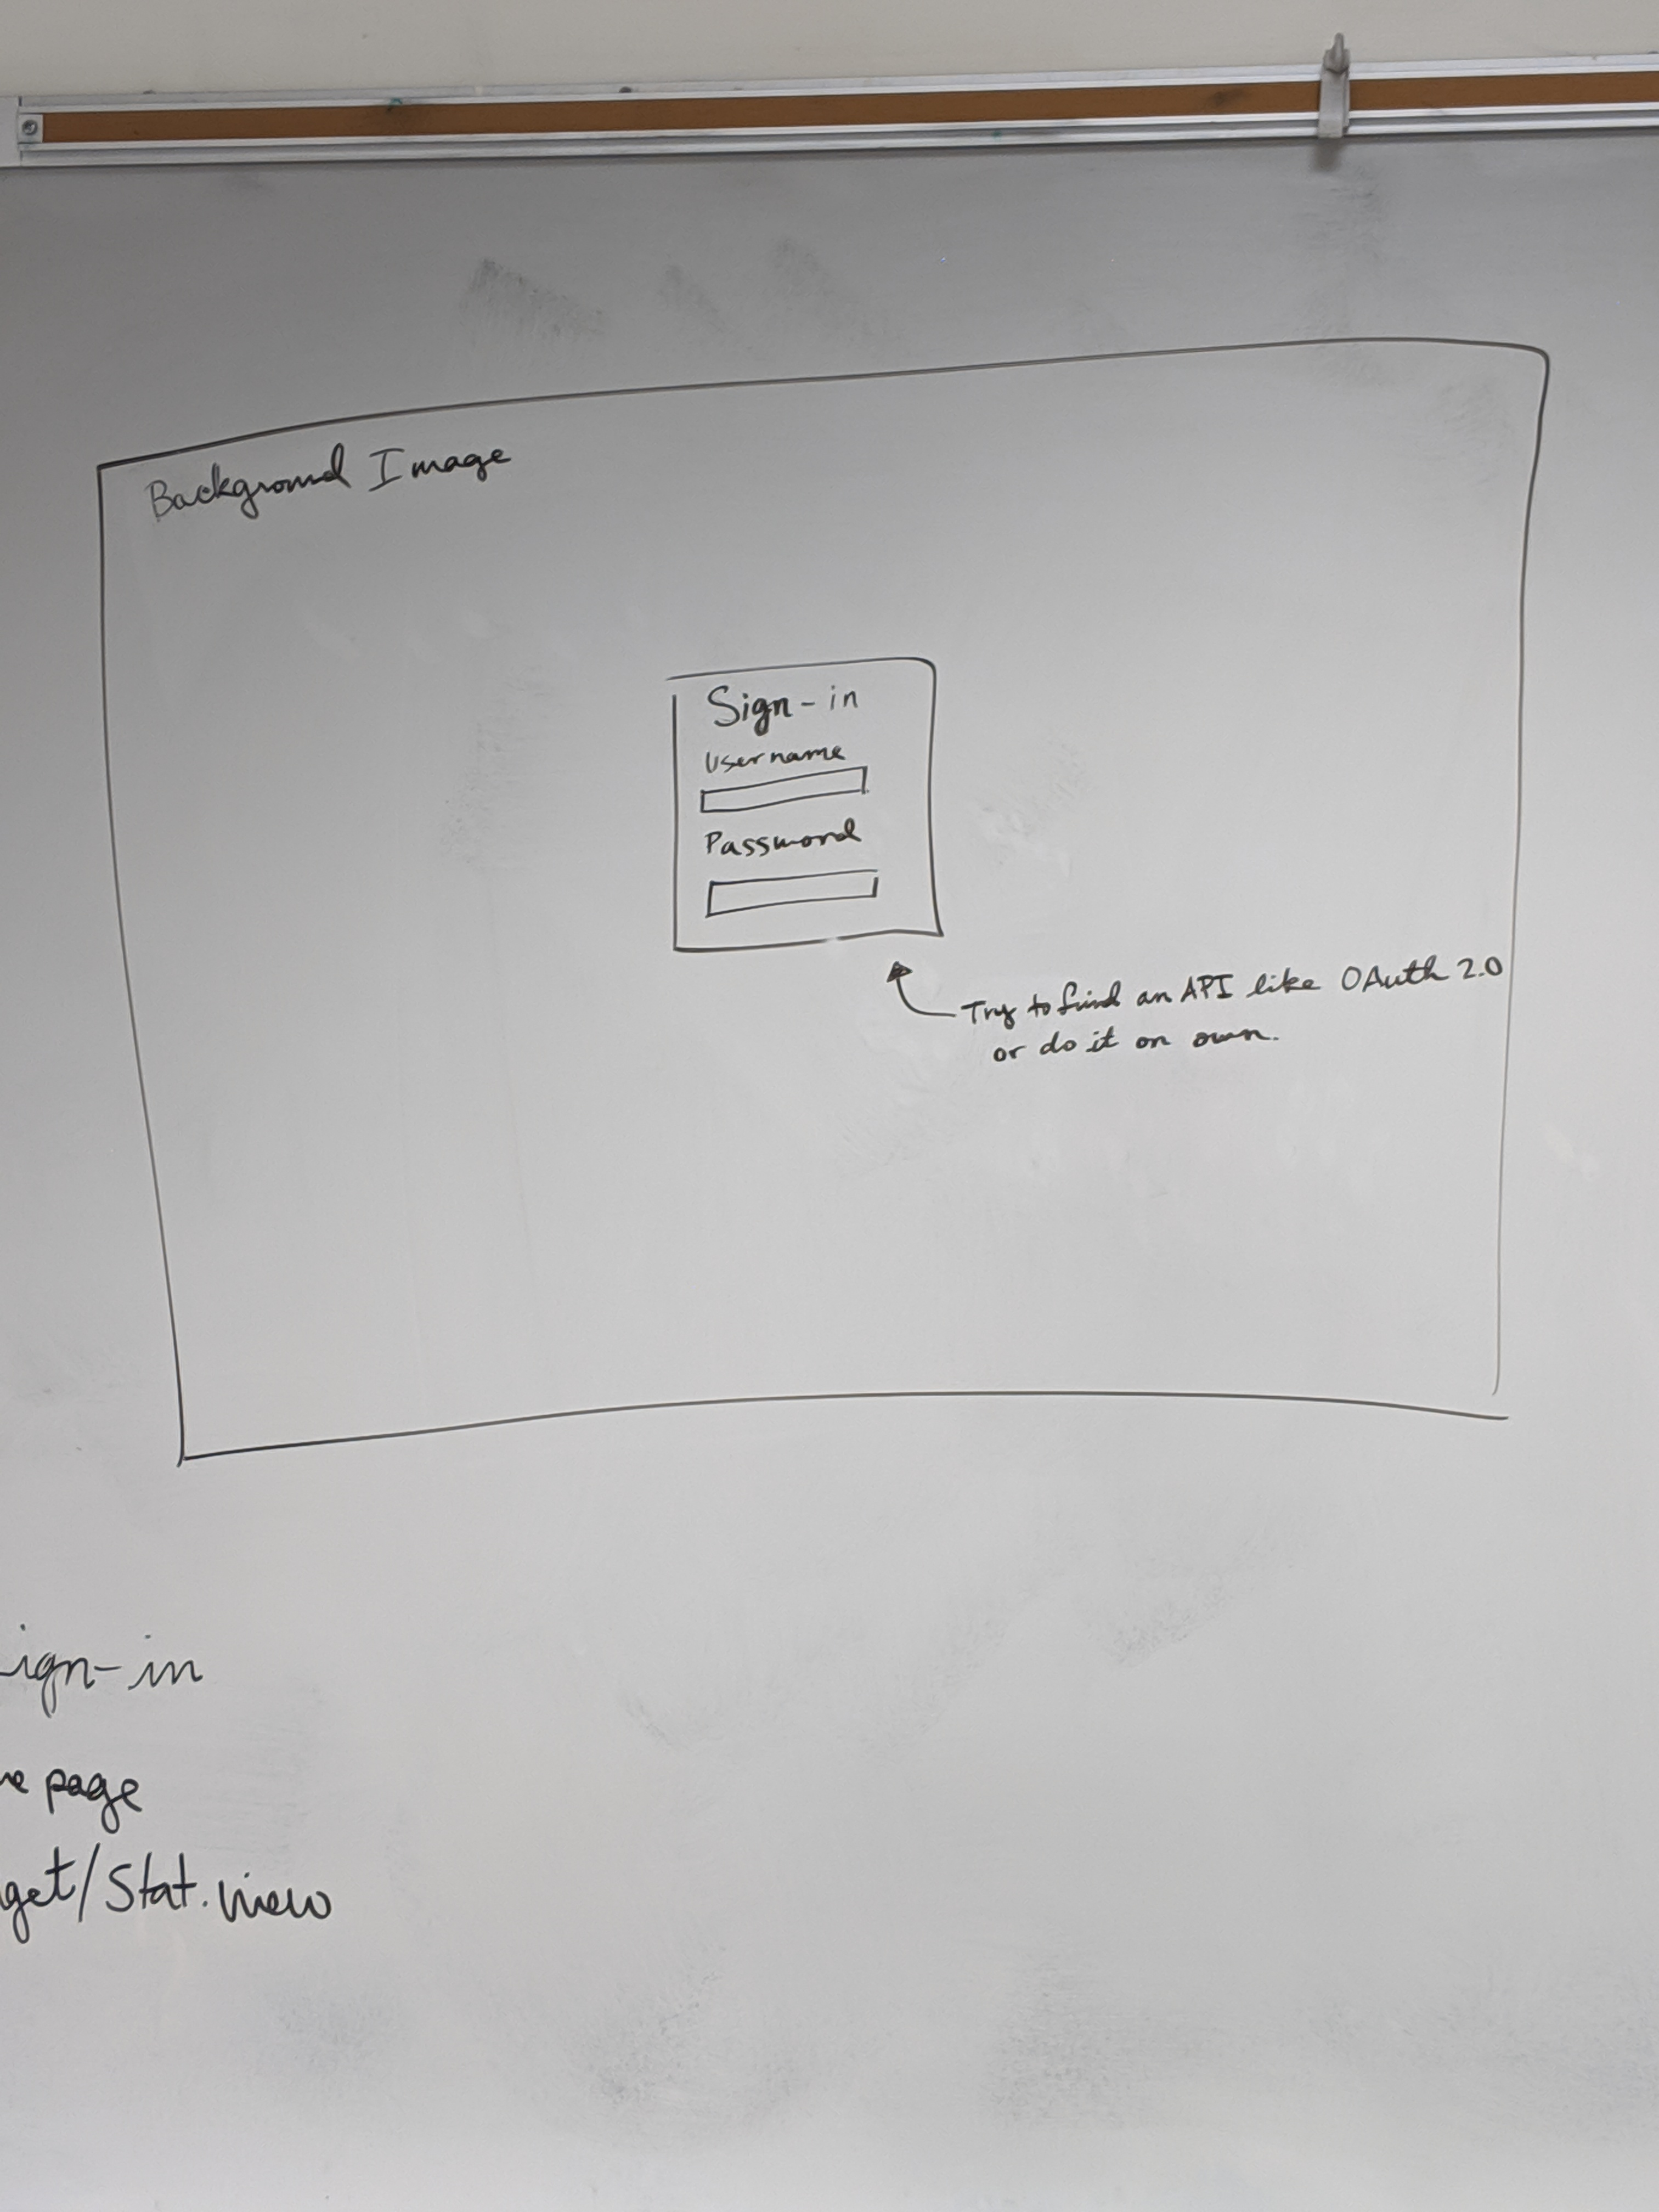
\includegraphics[scale = .05]{LoginIn.jpg}
\caption{The screen that the user will be greeted with and for case 3.}
\label{LoginScreen}
\end{minipage}%
\begin{minipage}{.5\textwidth}
\centering
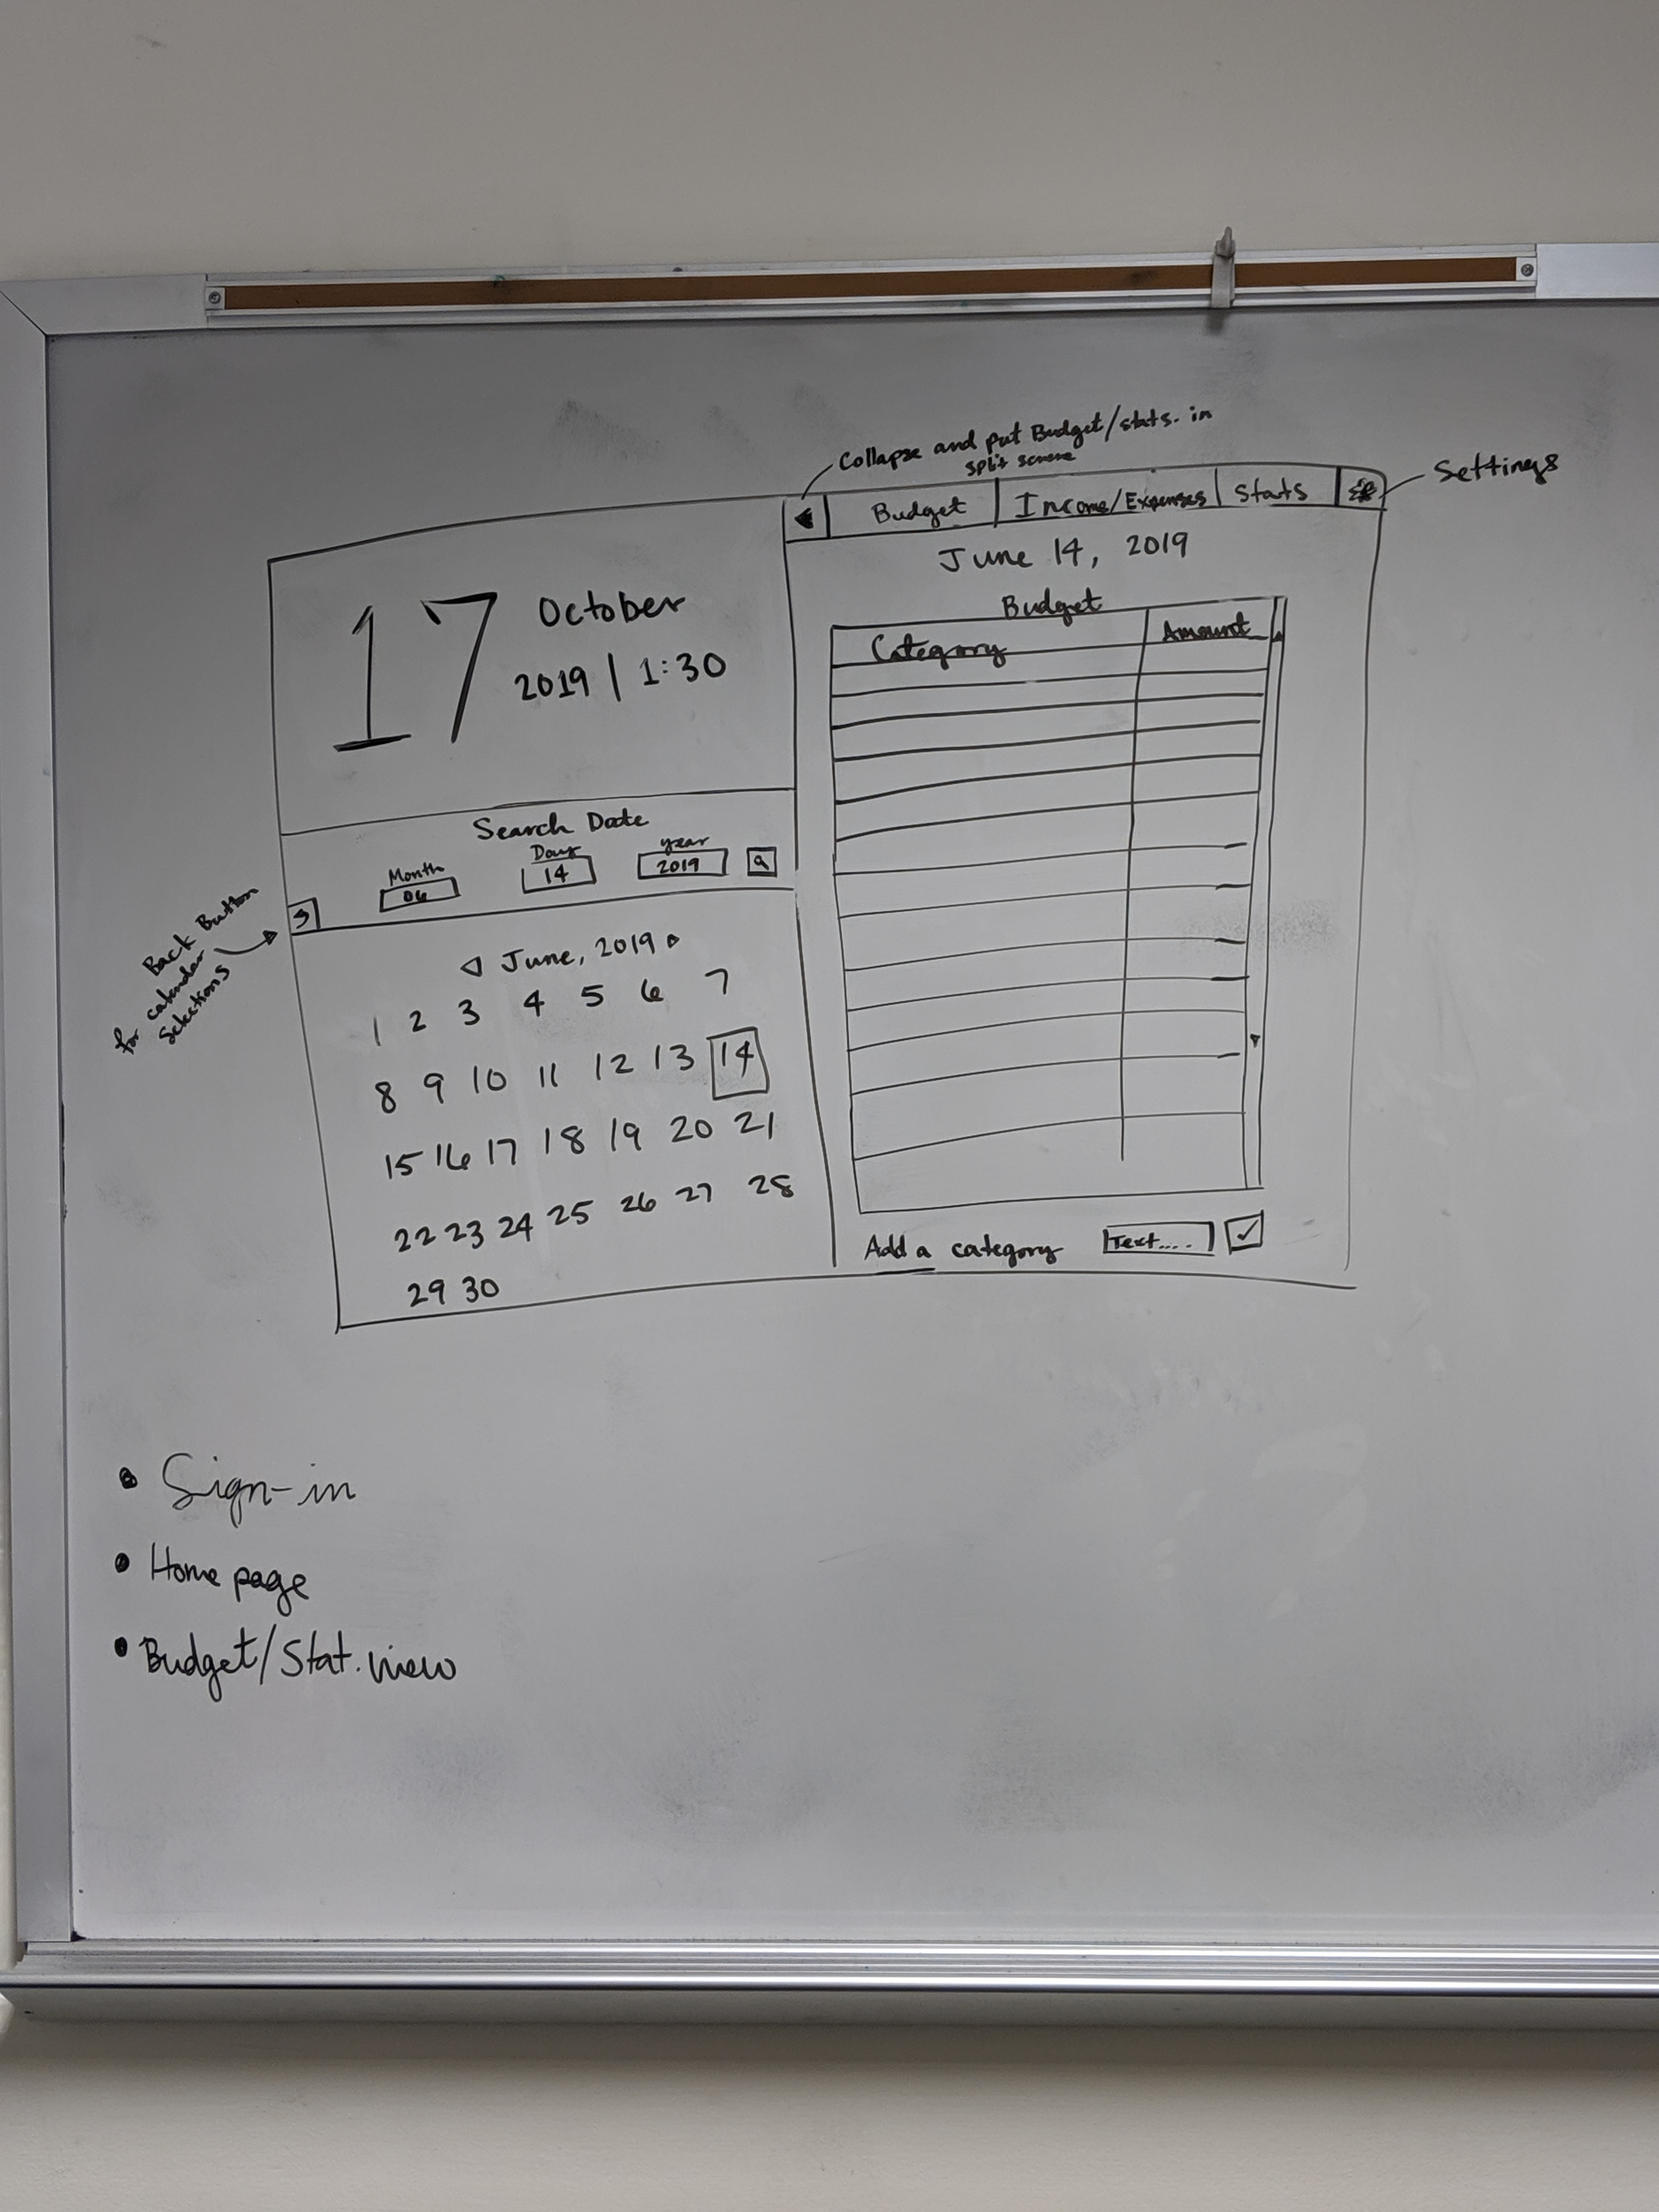
\includegraphics[scale = .05]{BudgetView.jpg}
\caption{Displays the budget information for selected time frame, and takes input (for example use case 2).}
\label{BudgetScreen}
\end{minipage}
\end{figure}


\begin{figure}[h]
\centering
\begin{minipage}{.5\textwidth}
\centering
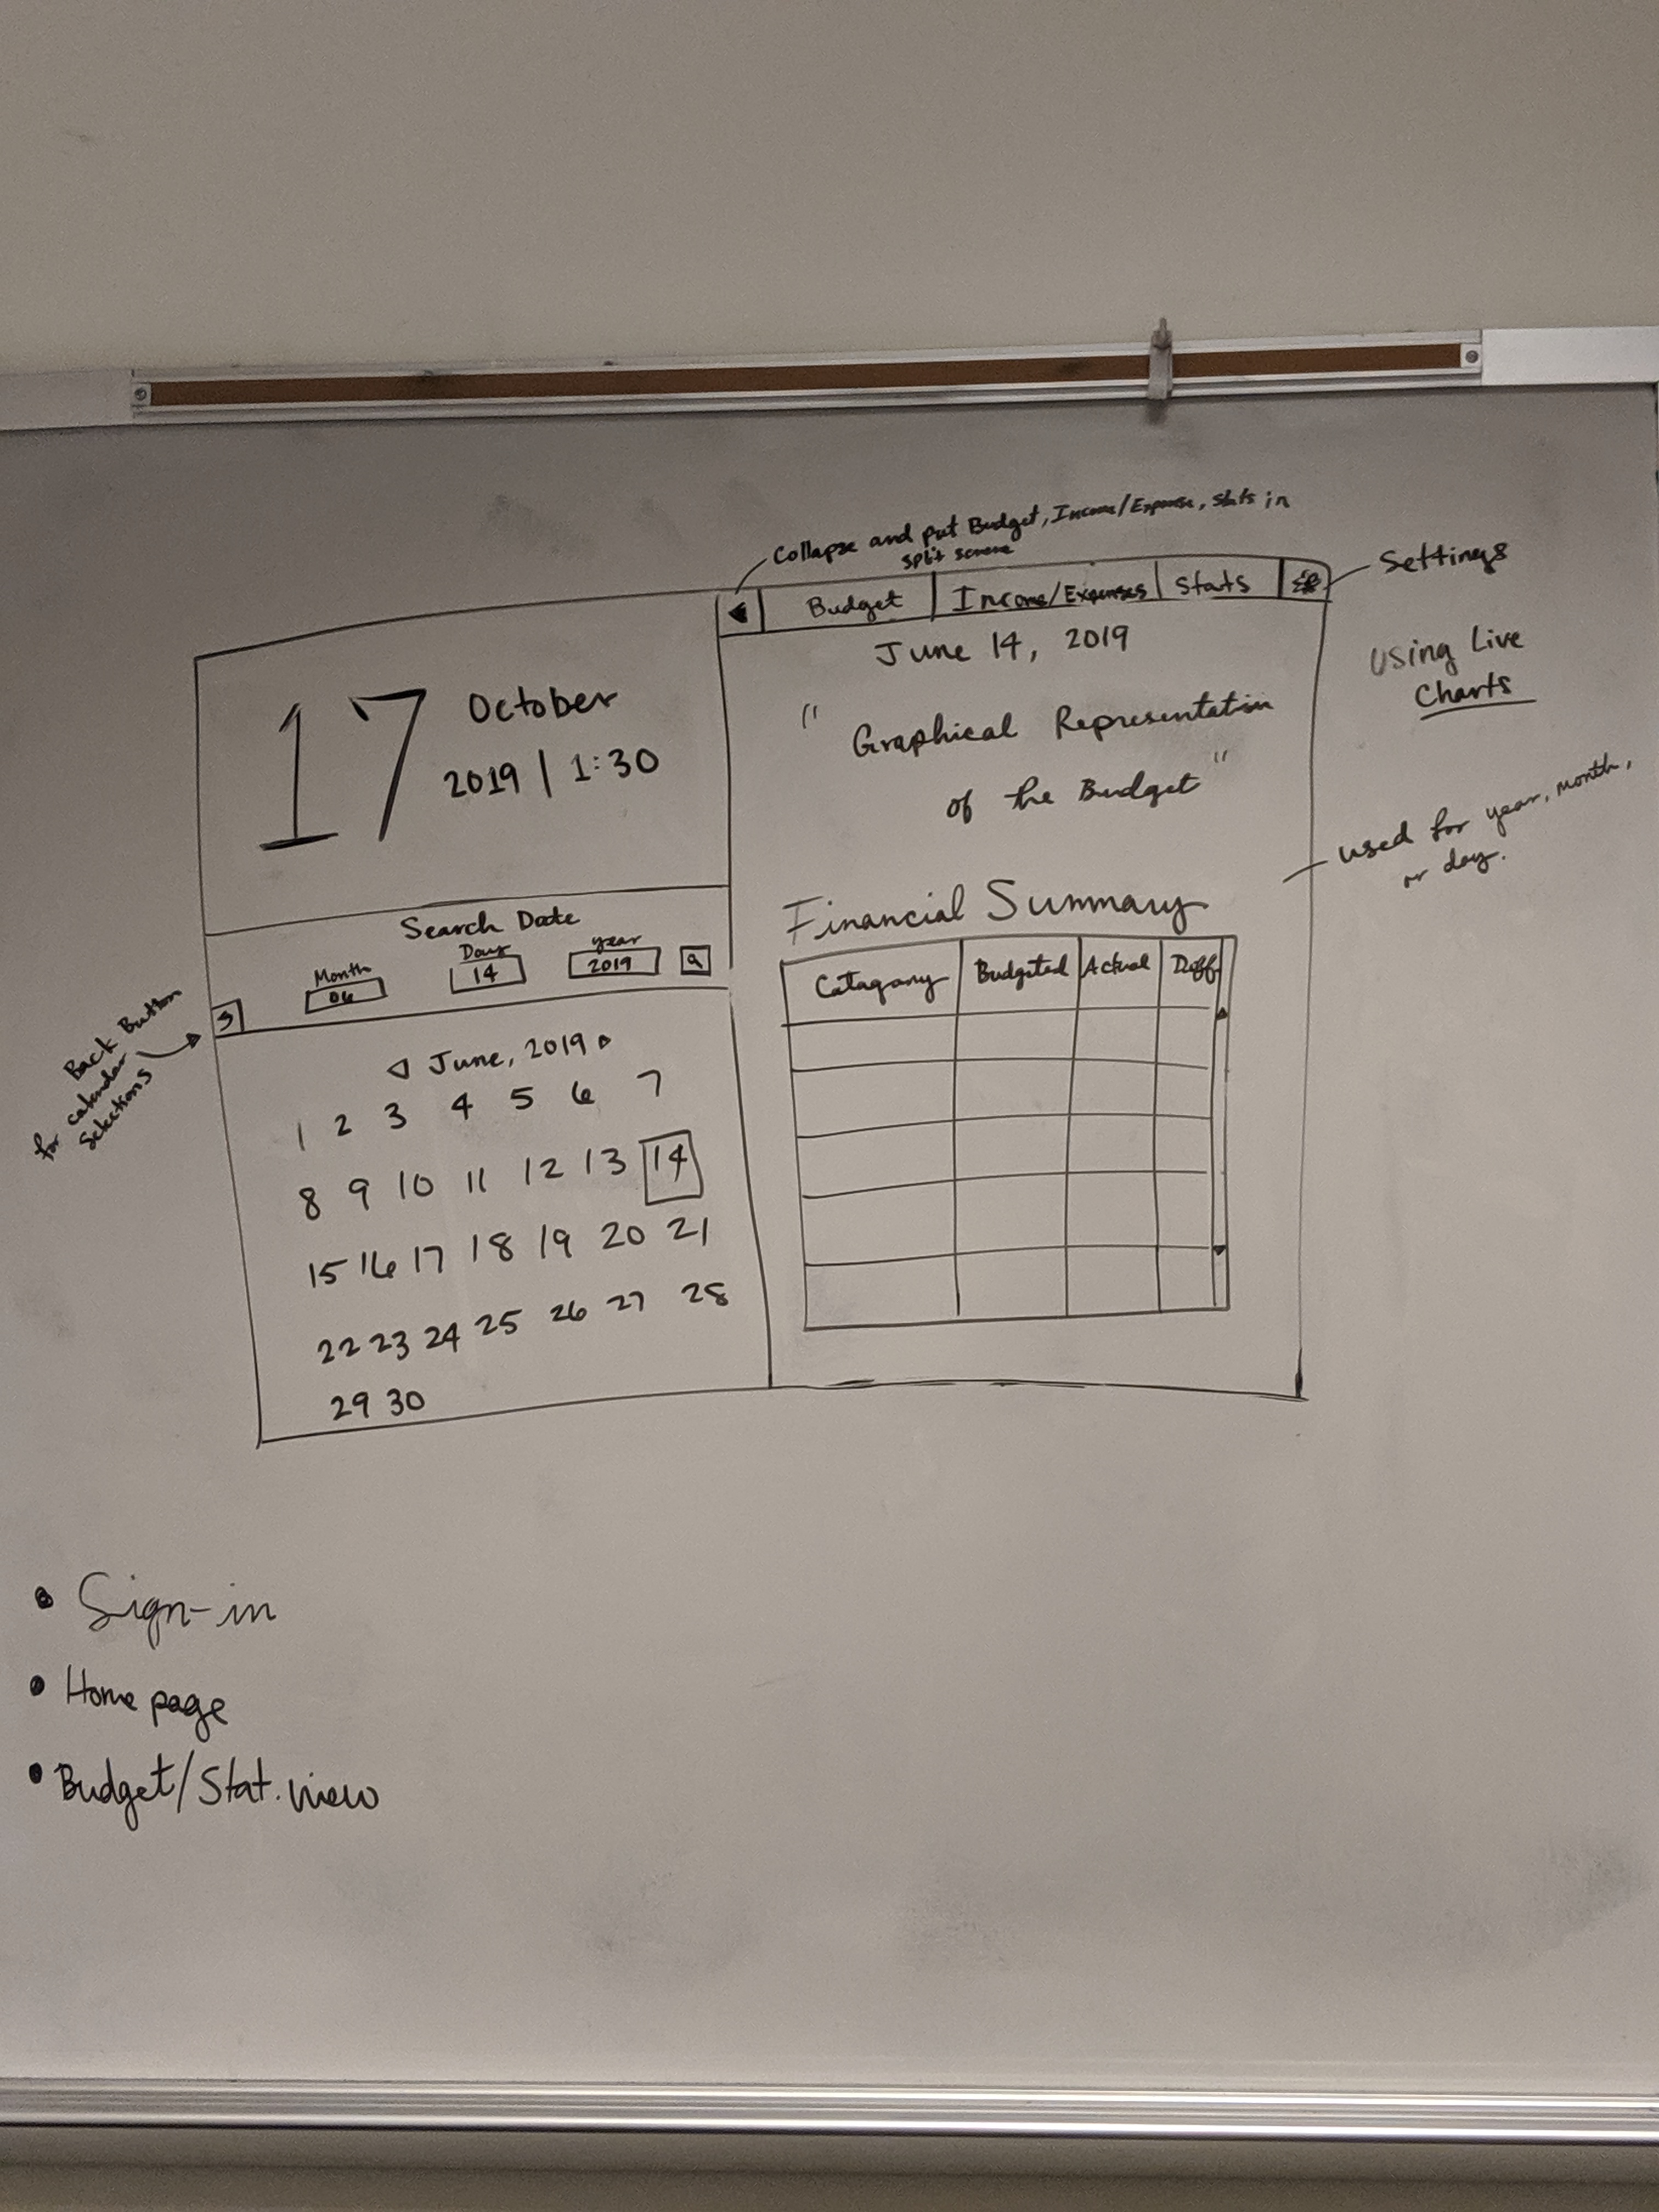
\includegraphics[scale = .05]{StatsView.jpg}
\caption{Displays the statistics for selected time frame.}
\label{StatsScreen}
\end{minipage}%
\begin{minipage}{.5\textwidth}
\centering
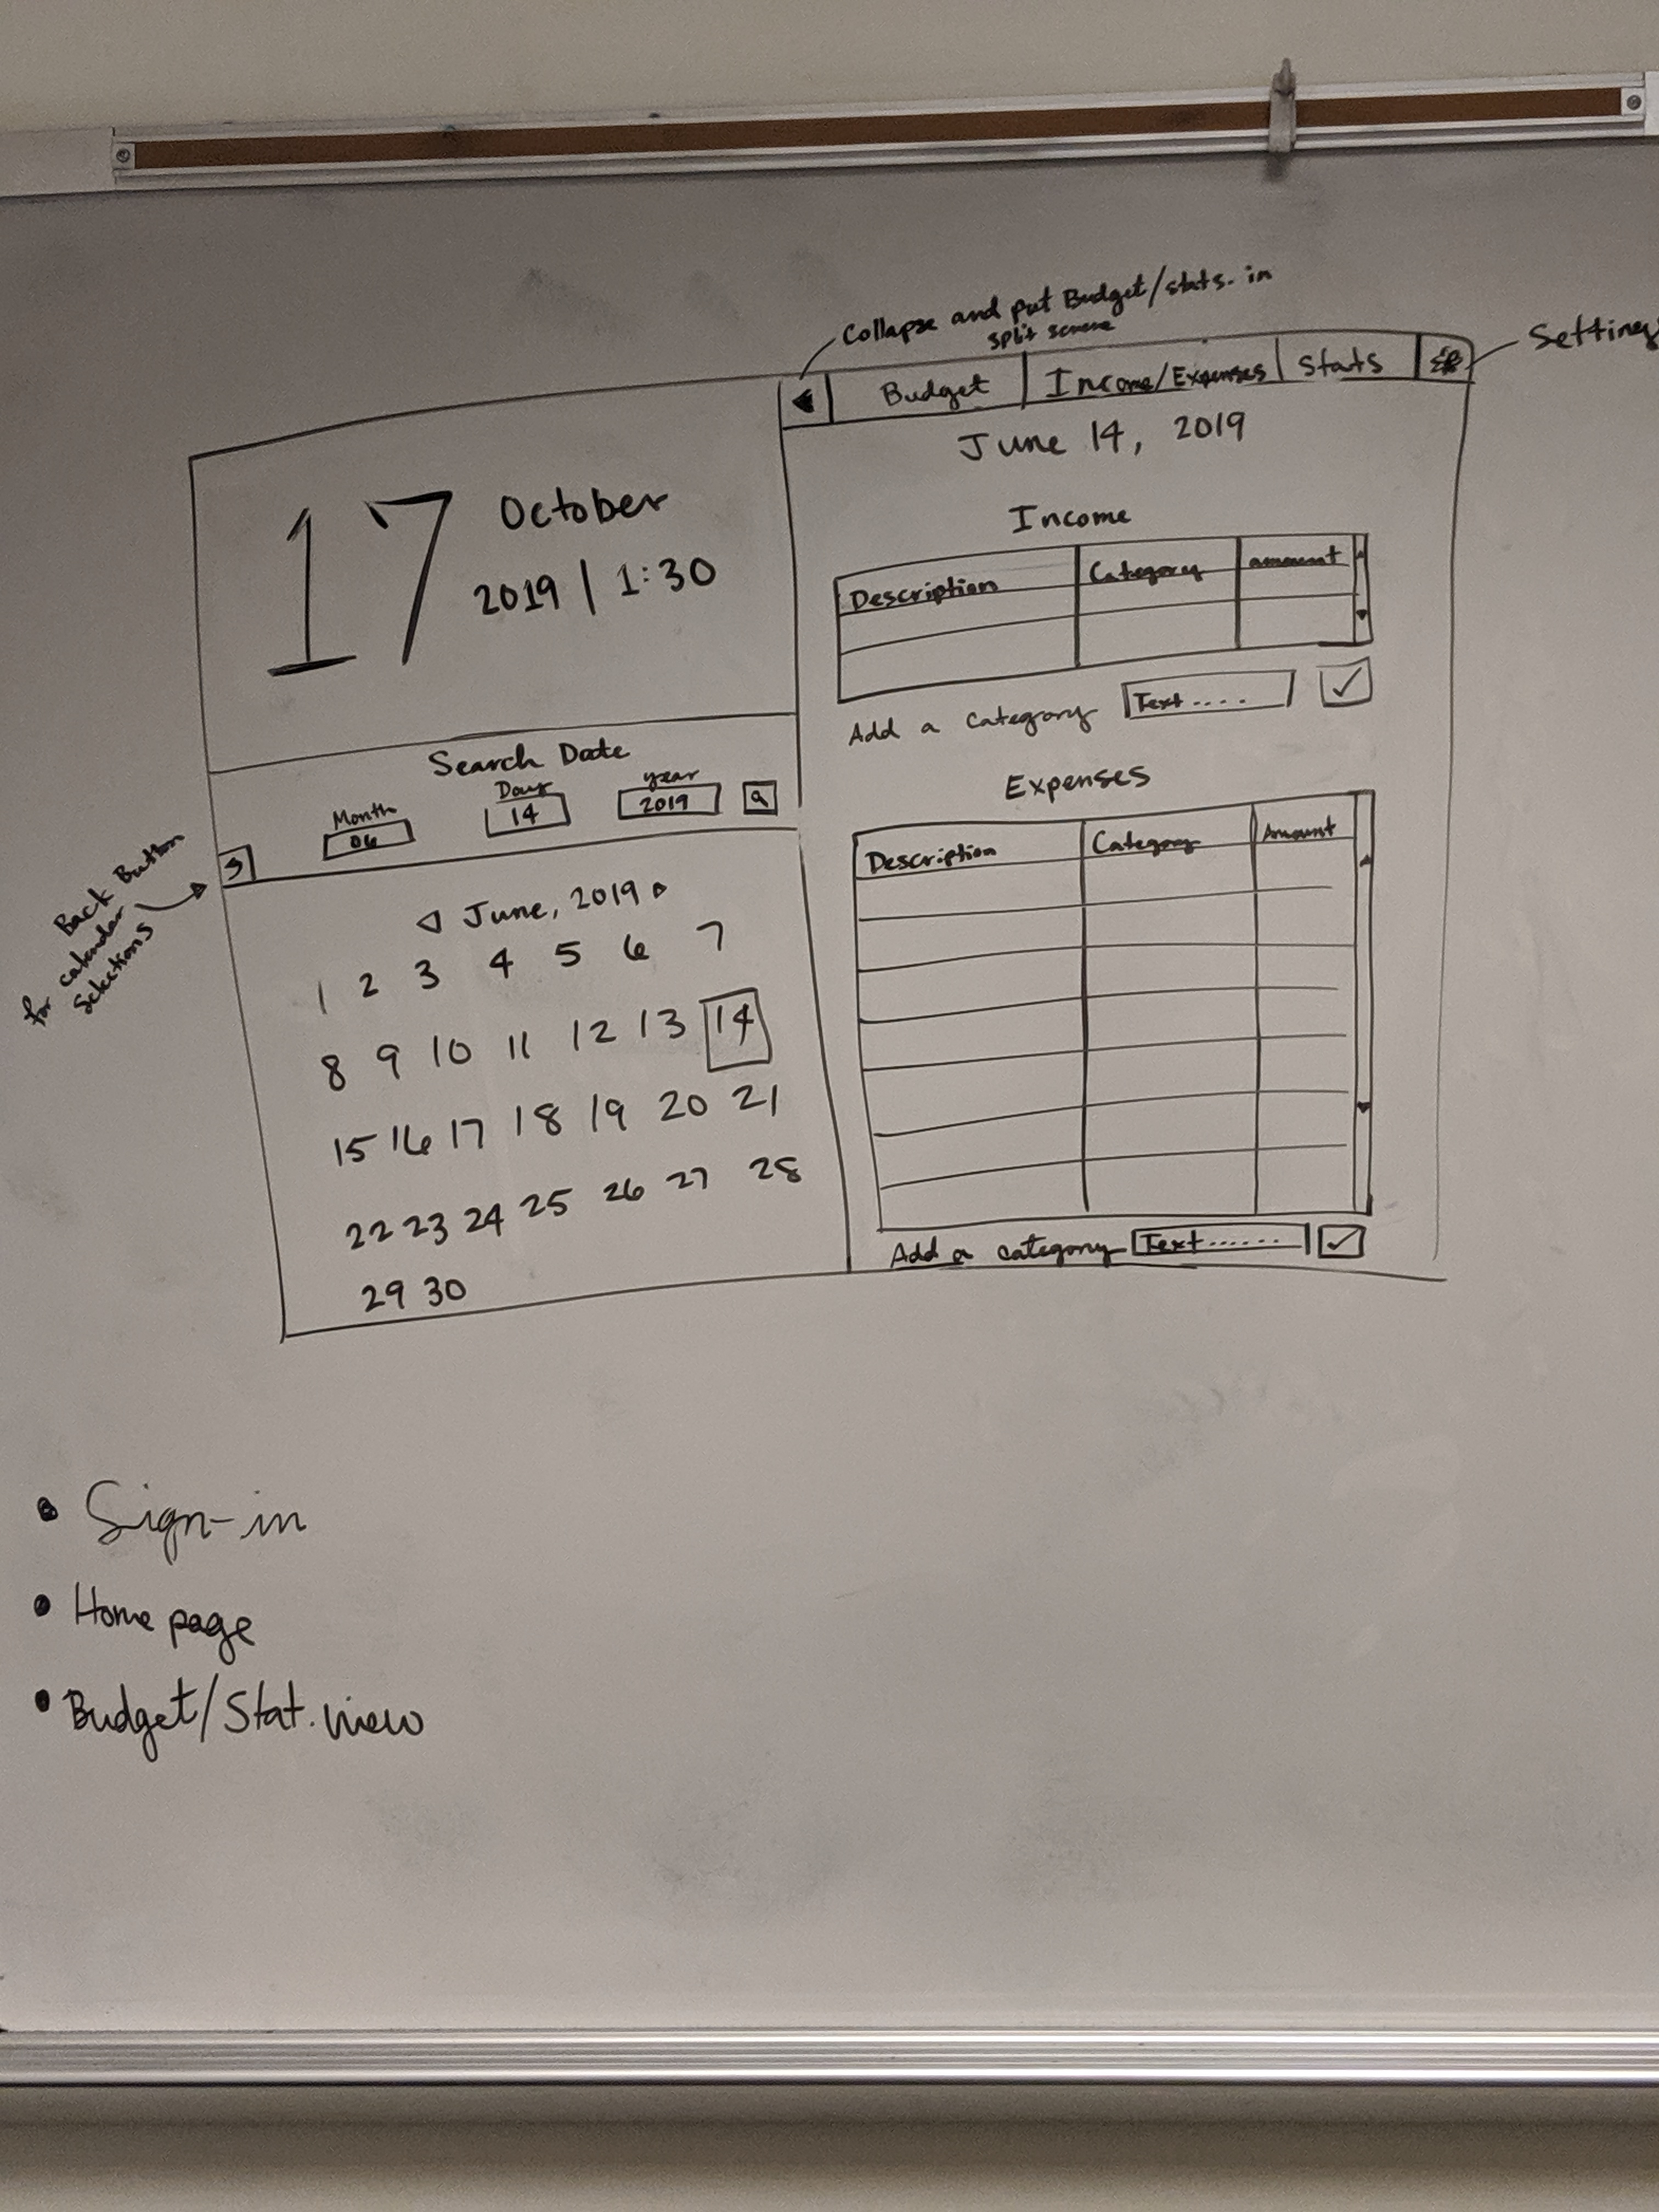
\includegraphics[scale = .05]{Income-Expenses.jpg}
\caption{Displays income and expenses for selected time frame, and takes input.}
\label{Income-ExpenseScreen}
\end{minipage}
\end{figure}


\section{Project Timeline}
Go back to your notes and look up a typical project development life cycle for the Waterfall approach.  How will you follow this life cycle over the remainder of this semester?  This will usually involve a chart showing your proposed timeline, with specific milestones plotted out.  Make sure you have deliverable dates from the course schedule listed, with a plan to meet them (NOTE: these are generally optimistic deadlines).

\section{Project Structure}
At first, this will be a little empty (it will need to be filled in by the time you turn in your final report).  This is your chance to discuss all of your design decisions (consider this the README's big brother).

\subsection{UML Outline}
Show the full structure of your program.  Make sure to keep on updating this section as your project evolves (you often start out with one plan, but end up modifying things as you move along).  As a note, while Dia fails miserably at generating pdfs (probably my fault), I have had much success with png files.  Make sure to wrap your images in a \texttt{figure} environment, and to reference with the \texttt{ref} command.  For example, see Figure \ref{cat2}.

\begin{figure}[ht!]
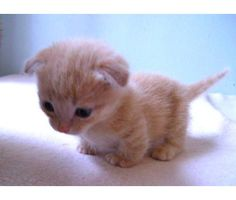
\includegraphics[scale=1.5]{cat2.jpg}
\caption{Your figures should be in the \emph{figure} environment, and have captions.  Should also be of diagrams pertaining to your project, not random internet kittens}
\label{cat2}
\end{figure}

\subsection{Design Patterns Used}
Make sure to actually use at least 2 design patterns from this class.  This is not normally part of such documentation, but largely just specific to this class -- I want to see you use the patterns!


\section{Results}
This section will start out a little vague, but it should grow as your project evolves.  With each deliverable you hand in, give me a final summary of where your project stands.  By the end, this should be a reflective section discussing how many of your original goals you managed to attain/how many desired use cases you implemented/how many extra features you added.

\subsection{Future Work}
Where are you going next with your project?
For early deliverables, what are your next steps?  (HINT: you will typically want to look back at your timeline and evaluate: did you meet your expected goals?  Are you ahead of schedule?  Did you decide to shift gears and implement a new feature?)
By the end, what do you plan on doing with this project?  Will you try to sell it?  Set it on fire?  Link to it on your resume and forget it exists?


\begin{thebibliography}{1}

\bibitem{IEEEhowto:kopka}
H.~Kopka and P.~W. Daly, \emph{A Guide to \LaTeX}, 3rd~ed.\hskip 1em plus
  0.5em minus 0.4em\relax Harlow, England: Addison-Wesley, 1999.

\end{thebibliography}

% biography section
% 
% If you have an EPS/PDF photo (graphicx package needed) extra braces are
% needed around the contents of the optional argument to biography to prevent
% the LaTeX parser from getting confused when it sees the complicated
% \includegraphics command within an optional argument. (You could create
% your own custom macro containing the \includegraphics command to make things
% simpler here.)
%\begin{IEEEbiography}[{\includegraphics[width=1in,height=1.25in,clip,keepaspectratio]{mshell}}]{Michael Shell}
% or if you just want to reserve a space for a photo:

%Ignore this for the lab

\begin{IEEEbiography}{Michael Shell}
Biography text here.
\end{IEEEbiography}

% if you will not have a photo at all:
\begin{IEEEbiographynophoto}{John Doe}
Biography text here.
\end{IEEEbiographynophoto}

% insert where needed to balance the two columns on the last page with
% biographies
%\newpage

\begin{IEEEbiographynophoto}{Jane Doe}
Biography text here.
\end{IEEEbiographynophoto}

% You can push biographies down or up by placing
% a \vfill before or after them. The appropriate
% use of \vfill depends on what kind of text is
% on the last page and whether or not the columns
% are being equalized.

%\vfill

% Can be used to pull up biographies so that the bottom of the last one
% is flush with the other column.
%\enlargethispage{-5in}



% that's all folks
\end{document}


